\documentclass[a4paper, titlepage, parskip]{scrartcl} 
% Format A4, mit Titelseite, mit Durchschuss (= Abstand zwischen Absätzen, statt Einrückung)
% KOMA-Script Grundklasse     texdoc scrguide

% Englisch mit Schriftkodierung mit Umlauten
\usepackage[USenglish]{babel}
\usepackage[T1]{fontenc}

% Mathematische Symbole etc.
\usepackage{textcomp,amsmath,amssymb}

% Standard Graphik Paket
\usepackage{graphicx}

% kann UTF-8 source lesen
\usepackage[utf8]{inputenc}

% Definition environment
\usepackage{amsthm} 
\theoremstyle{plain}
\newtheorem{definition}{Definition}
\theoremstyle{definition}
\newtheorem{quotecaption}{Quote}
% force figures inline with [H]
% \usepackage{float}

% highlight text
% \usepackage{xcolor}

% cite in italics
\newcommand*{\itcite}[1]{\glqq\textit{#1}\grqq} 

% center without vertical spacw
\newenvironment{nscenter}
 {\parskip=0pt\par\nopagebreak\centering}
 {\par\noindent\ignorespacesafterend}

% bibtex
\usepackage{url}
\bibliographystyle{plaindin}      % BibTeX Styles nach Norm DIN 1505

% Abstract Breite
% https://tex.stackexchange.com/questions/151583/how-to-adjust-the-width-of-abstract
\renewenvironment{abstract}[1]
 {\small
  \begin{center}
  \bfseries #1\vspace{-.6em}\vspace{0pt}
  \end{center}
  \list{}{
    \setlength{\leftmargin}{.6cm}%
    \setlength{\rightmargin}{\leftmargin}%
  }%
  \item\relax}
 {\endlist}

% Unterschriftzeile
% https://tex.stackexchange.com/questions/183698/signature-line-with-dots-and-name-below
\newcommand{\sign}[1]{
  \begin{tabular}[t]{@{}l@{}}
  \makebox[2.5in]{\dotfill}\\
  \strut#1\strut
  \end{tabular}
}

% Titelseite
\titlehead{

\includegraphics{img/hpi_logo_cmyk_wb_sl2}
} \subject{Bachelor Thesis}
\title{Evaluation of Entity Linking Models on Business Data
\\ \bigskip 
\large{Evaluierung von Entitätsverknüpfungsmodellen auf Unternehmensdaten}}
\author{Jan Ehmüller\\{\small{\url{jan@ehmueller.de}}}}
\date{\today}
\publishers{
Information Systems Group\\
~\\
\textbf{Supervisors}\\
Prof. Dr. Felix Naumann\\
Toni Grütze\\
Michael Loster}

\begin{document}
\maketitle

\newpage
\begin{abstract}{Abstract}
I will write this section at last.
\end{abstract}

\newpage
\begin{abstract}{Zusammenfassung}
Und hier steht das gleiche nochmal auf deutsch.
\end{abstract}
\newpage
%{\small\tableofcontents}
\tableofcontents
\addtocontents{toc}{\setcounter{tocdepth}{2}}
\newpage
\section{Ambiguous Business Aliases}
\label{sec:IntroABA}
The graph of Germany's corporate landscape contains nodes, which are businesses, and edges, which are the relations between businesses. Information about businesses is extracted from structured knowledge bases such as Wikidata and DBpedia. They describe the businesses themselves but contain incomplete information about the relations between them. These relations are described in unstructured texts like Wikipedia or newspaper articles. They need to be extracted from these unstructured texts to be transformed into an edge of the graph.\par
For our approach to extract a relation between two businesses they must first be mentioned in the same sentence. Then both of these mentions need to be found and linked to the entities representing these businesses. Finding these mentions is called \textit{Named Entity Recognition} (NER). They must then be linked to the correct entities in the knowledge base. This step is called \textit{Entity Linking} (EL). The last step is to extract the relation between the two businesses from the sentence, which is called \textit{Relation Extraction} (RE). Our approach combines NER and EL into a single step and transforms it into a classification problem. These resulting two steps, the combination of NER and EL and the RE step, make up the Information Extraction step in the pipeline described in the Introduction. Janetzki \cite{janetzki} describes the creation of our knowledge base and the extraction of features used to classify mentions. This work evaluates the quality of the features and different classification models. Schneider \cite{schneider} describes and evaluates different Relation Extraction methods.\par
Section \ref{sec:RelatedWork} covers related work in the field of both NER and EL and especially related work about recognizing and linking business entities and efficient NER and EL on millions of documents in acceptable time. Section \ref{sec:NEL} describes the used approach that combines both NER and EL. After that different classification models and configurations are compared and evaluated in Section \ref{sec:ModelEval}. Section \ref{sec:FeatureEval} evaluates the features used to train the classifier. These features are described in detail by Janetzki \cite{janetzki} and Grütze et al. \cite{coheel}. Section \ref{sec:NELEval} discusses the performance and quality of this approach when annotating millions of newspaper articles. Finally, Section \ref{sec:Conclusion} concludes this thesis and describes possible improvements that could be done in the future.

\newpage
% (1 Seite)
\section{Related Work (1 Seite)}
Einmal Paper zu NER citen und kurz sagen was sie machen und dann auch zu NEL (u.a. CohEEL). Dann sagen was wir anders machen.


	\subsection*{Alias Generation to Improve Company Recognition in Text}
	\begin{itemize}
		\item ähnliches Ziel (NEL von Unternehmen)
		\item arbeitet mit dem "Wortstamm" der Aliase
		\item kann so auch nicht bekannte Vorkommen eines Unternehmensaliases finden
		\item dadurch ist Disambiguierung aber schwieriger, da z.B. Unternehmensformen aus dem Namen entfernt werden
		\item (eventuell gab es keine Disambiguierung?)
	\end{itemize}

	\subsection*{CohEEL}
	\begin{itemize}
		\item nur NEL und kein NER
		\item benutzt Seed und Candidate Alignments und kombiniert diese mit JNE (und Random Walks)
		\item benutzt sehr ähnliche first order features
		\item benutzt die selben higher order features
		\item läuft auch verteilt (Flink)
	\end{itemize}
\newpage
% (2-3 Seiten)
\section{Named Entity Linking}
\label{sec:NEL}
This section describes the classification problem combining both NER and NEL and its solution. Given an input text, all mentions of businesses should be recognized and linked to the correct business while other mentions of named entities should be ignored. Quote \ref{quote1} shows two example sentences about automobile businesses. Only the bold named entities are businesses and should be linked to entities in the knowledge base. Usual NER approaches however (needs citation) recognize all named entities, which in this example are businesses as well as non-businesses. Since the linked entities are used to extract relationships between businesses they must only be businesses. To solve this problem a classifier is trained using the German Wikipedia and its hand annotated links as knowledge base. The following sections describe the how the classifier is trained and how it is then used to annotate documents.\\
\begin{nscenter}
	\fbox{\parbox[c][74pt]{\textwidth}{Sechs Top-Manager von \textbf{GM}, darunter \underline{Robert A. Lutz} sowie \underline{Carl-Peter Forster}, welcher als Group Vice President für das Europageschäft zuständig ist, trennten sich Anfang Mai 2009 von ihren gesamten Anteilsscheinen.\\PSA-Chef \underline{Carlos Tavares} hatte zugesagt, \textbf{Opel} als deutsches Unternehmen zu erhalten. Er hatte aber zugleich angekündigt, \textbf{Opel} müsse sich im Fall einer Übernahme durch \textbf{PSA} weitgehend aus eigener Kraft sanieren.}}
	\begin{quotecaption}
	Two example sentences containing highlighted named entities. Business entities are bold and other non-business entities are underlined.
	\label{quote1}
	\end{quotecaption}
\end{nscenter}

\subsection{Classifier training}
The German Wikipedia has around 3.6 million pages and around 38 million links occurring in the text. Only a fraction of these contains relevant data which would be useful to train a classifier to link business entities. To reduce this massive amount of data to a smaller, more relevant dataset the links are filtered with the help of Wikidata. Wikidata is a structured knowledge base derived from Wikipedia. Using its ontology with the pages in Wikipedia can be reduced to only the pages about businesses. Let $W$ be the set of all Wikipedia pages and $W_{business} = \{ P \in W | P \text{ is tagged as business in Wikidata} \}$.
\begin{definition}
A \textbf{link} l = (P,i,a,P') is the textual occurrence of an alias a in position i within Wikipedia page P and linking to the Wikipedia page P'.
\label{link}
\end{definition}
Using this smaller set of business pages the relevant links can be reduced as well. Let $L$ be the set of all links occurring in Wikipedia and $L_{business} = \{ l = (P,i,a,P') \in L | P' \in W_{business} \}$. Using this smaller set of links pointing to the pages of businesses the possible aliases of businesses can be extracted. Let $A$ be the set of all aliases links in Wikipedia have and $A_{business} = \{ a \in A | \exists l \in L_{business}: l \text{ has alias } a \}$. Next $L_{business}$ is expanded by selecting every link with an alias that has the possibility to link to a business. These links $L'_{business} = \{ l \in L | \exists a \in A_{business}: l \text{ has alias } a \}$ comprise the relevant links that will be used to train the classifier.\par
Due to the readability of the Wikipedia pages, however, there are two issues with these links: the mention of an entity on its own page is not linked to the page and usually only the first occurrence of an entity's mention is linked. To solve these two issues the links on a given Wikipedia page P need to be extended. First, all links occurring on page p are extracted into the set $L_P = \{ l \in L'_{business} | l \text{ occurs on page } P\}$. These links are then used to creating the set $P_P = \{ P' \in W | \exists l \in L_P: l \text{ links to page } P' \} \cup \{P\}$ containing all pages mentioned on page P and the page itself. Using $P_P$ all links linking to these pages are aggregated into $L'_P = \{ l \in L'_{business} | \exists P' \in P_P: l \text{ links to } P' \}$. The aliases $A_P = \{a \in A_{business} | \exists l \in L'_P: l \text{ has alias } a \}$ are tokenized and these tokens are used to create a trie. In this trie each leaf represents a token of an alias. For example, the alias \itcite{Volkswagen AG} would be represented by the leaves \itcite{Volkswagen} and \itcite{AG}. With this trie all occurrences of the aliases $A_P$ on page $P$ are found and transformed into extended links $LE_P = \{ l_e = (P, i, a, W_a) | a \in A_P \land a \text{ occurs on page } P \text{ in position } i \land \nexists l \in L_P: l \text{ occurs in position } i \}$.
\begin{definition}
An \textbf{extended link} $l_e$ = (P,i,a,$W_a$) is the textual occurrence of an alias a in position i within Wikipedia page P and possibly linking to the Wikipedia pages $W_a = \{ P' \in W | \exists l \in L: l \text{ links to page } P' \land l \text{ has alias } a \}$.
\label{extendedlink}
\end{definition}
These extended links are then transformed into actual links $LE'_P$ extending $L_P$ by applying a partial function $f_{LE}$.
This function transforms an extended link $l_e = (P,i,a,W_a)$ into a link $l = (P,i,a,P')$ if and only if $W_a$ has only a single element $P'$ or there is only one page $P' \in W_a$ for which there are at least two links with alias $a$ and these links make out at least 90\% of all links pointing to $P'$. $L_{P_{positive}} = LE'_P \cup L_P$ then makes up all the links on page $P$ used for the classifier training.\par
The links in $L_{P_{positive}}$ all represent true annotations. But the classifier is also supposed to disambiguate true annotations and false, non-business, ones, as seen in Quote \ref{quote1}. Thus the training set needs to be extended by false annotations. These are found by searching for the occurrences of known aliases on Wikipedia page P which were not linked by a human. The assumption is that since these entities were not linked by a human that they are false in this context.
\begin{definition}
A \textbf{trie alias} t = (P,i,a) is the textual occurrence of an alias a in position i within Wikipedia page P found by using a trie of known aliases.
\label{triealias}
\end{definition}
These occurrences are found by creating a trie from the tokenized aliases in $A_{business}$ which is then used to find re-occurrences of known aliases. In the case of overlapping occurrences, only the longest occurrence is used. An example of such an overlap would be the sentence \itcite{Die Audi AG sitzt in Ingolstadt.}. Here the trie would find occurrences of both \itcite{Audi} and \itcite{Audi AG} but only the longest occurrence will be considered. These trie aliases make up the set $L_{P_{negative}} = \{ t = (P,i,a) | a \text{ occurs on page } P \text{ in position i } \land \nexists l \in L_{P_{positive}}: l \text{ occurs in position } i \}$ containing the false annotations on page P.\par
The number of trie aliases found is several times higher than the number of links and extended links per page. This can cause problems if there are so many more false annotations that the classifier just classifies every entry as wrong because it is still right in over 99\% of the cases. The approach used to reduce the number of trie aliases is to remove stop words and symbols because they will be almost never used to refer to businesses in newspaper articles.\par
To train the classifier the links and trie aliases of the small subset of Wikipedia pages $W_{business}$ are used. Every link in $L_{P_{positive}}$ and every trie alias in $L_{P_{negative}}$ is transformed into a number of feature entries. The possible pages a given alias $a$ can point to are $P_a = \{ P \in W | \exists l \in L_{business}: l \text{ has alias } a \land l \text{ points to page } P \}$.
\begin{definition}
A \textbf{feature entry} $f_e$ = (P,i,a,P',F) represents an alias occurring on Wikipedia page P in position i and possibly pointing to a Wikipedia page P' with a set of generated features F used to train a classifier.
\label{featureentry}
\end{definition}
This set of features $F$ contains three first order features and six higher order features as described by Janetzki \cite{janetzki}. These first order features are the link score, the page score and the link context score. Given a feature entry $f_e = (P,i,a,P',F)$, the link score signifies how likely it is, that the alias $a$ links to any page. It is, therefore, the same for every feature entry generated from one link or trie alias. The page score represents the likelihood that given the alias a links to any page links specifically to page P'. The link context score shows the similarity of the words around alias a on page P in position i to the words on page P'. Because the link score is equal for all feature entries generated from one link or trie alias, the higher order features are only generated for the page score and the link context score. They are as described by Grütze et al. \cite{coheel} the rank, $\Delta top$ and $\Delta succ$. They describe the relationship between the feature entries generated by a single link or trie alias. The rank is an integer ranking of the values of the feature, which is defined by the partial order $\geq$. This means that the highest value of the feature has the lowest and best rank of 1 while the lowest value has the worst rank of $n$, with $n$ being the number of feature entries generated for a specific link or trie alias. $\Delta top$ describes the difference between the current feature entry to the one with rank 1. In the case of the feature entry with rank 1 its value is $\infty$. $\Delta succ$ describes the difference to the feature entry with the next higher (worse) rank. In the case of the worst feature entry with rank $n$ its value is also $\infty$.\par
Around 545 million feature entries containing these features were used to train the classifier. Different classification models will be evaluated in section 4 and the first and higher order features will be evaluated in section 5.
	% \begin{itemize}
	% 	\item trainieren auf den Links in der Wikipedia
	% 	\item extended links als Erweiterung der normalen Links
	% 	\item Trie Hits als negatives für das Training
	% 	\item (hier die Features erklären anstatt in der nächsten section)
	% \end{itemize}

\subsection{Annotation of Newspaper Articles}
The process of annotating newspaper articles is very similar to the training process. Given an article D, the first task is to find possible mentions of businesses. This is done with the trie built using $A_{business}$. These trie aliases are again filtered by removing stop words and symbols since they are assumed to almost never reference a business. As just described a number of feature entries are then generated from every trie alias found in article D. They are then classified using the trained classification model. Because one trie alias generates multiple feature entries which are classified independently it is possible that multiple feature entries generated from one trie alias are classified as links to businesses. When this happens there is no way to rank the multiple possible entities since the classifier just does a boolean decision. Because of that, these collisions are filtered and the alias is not linked to any entity. %These cases will be included in the evaluation of the classification models and features in the following sections.
	% \begin{itemize}
	% 	\item finden mögliche Aliase einer Entität über die Wikipedialinks (Wikipedia = Knowledge Base)
	% 	\item filtern Wikipedia Entitäten anhand der Wikidata Ontologie auf Unternehmen
	% 	\item suchen nach allen Vorkommen aller Aliase/Mentions dieser Unternehmen in Fließtexten anhand eines Prefix-Trees (Trie)\\
	% 	(Trie eventuell noch genauer erläutern?)
	% 	\item entfernen Stopwords und Symbole
	% 	\item für jedes Mention gucken wir uns an welche Alignments es laut Wikipedia geben kann
	% 	\item für jedes alignment werden drei first order features berechnet und für zwei dieser auch higher order features\\
	% 	(Jonathan)
	% 	\begin{itemize}
	% 		\item link score: wie wichtig das Mention ist (gleich für alle Alignments)
	% 		\item entity score: wie wahrscheinlich dieses Alignment in der Wikipedia ist
	% 		\item context score: wie ähnlich der Kontext der Mention und die Wikipedia Seite des Alignments sind
	% 	\end{itemize}
	% 	\item kurze higher order feature Erläuterung (Jonathan)
	% 	\item klassifizieren jedes Alignment
	% 	\item wenn für ein Mention mehrere Alignments als wahr klassifiziert wurden, werfen wir die Mentions weg, da wir nicht wissen welches Alignments korrekt ist
	% \end{itemize}

\newpage
% (4 Seiten)
\section{Evaluation of the Classification Models}
\label{sec:ModelEval}
This section first evaluates different classification models with three quality measures. These are the Precision $P$, the Recall $R$ and the $F_{\beta}$-Score, which are defined in Definition \ref{def_prf}. Specifically, the $F_1$-Score is used, which is the harmonic mean of the Precision and the Recall and thus favors neither. Then the class thresholds of a Random Forest model is evaluated to see whether or not it can be used to create both a high Precision and a high Recall model to create seed and candidate alignments as described by Grütze et al. \cite{coheel}. These quality measures are unrealistic for the use case of this approach as they do not take the collisions described in Section \ref{sec:NEL} into account. That's why they will be compared with adjusted quality measures, which take the collisions into account, at the end of this section.\par
Let $T$ be the set containing the feature entries to be classified. Each feature entry has a label containing the result (positive or negative) the classifier should predict. A positive label on a feature entry means that its alias links to its entity and that it should be classified as such. A negative label means that the feature entry should not be classified as links because either it's not a link at all or it links to the wrong entity. The subsets $T_{TP}$, $T_{FP}$ and $T_{FN}$, which are used to calculate the quality measures, are defined as follows.\\
\begin{nscenter}
	$T_{TP} \subset T$, where $\forall f_e \in T_{TP}: f_e$ is labeled positive $\land$ $f_e$ is classified positive\\
	$T_{FP} \subset T$, where $\forall f_e \in T_{FP}: f_e$ is labeled negative $\land$ $f_e$ is classified positive\\
	$T_{FN} \subset T$, where $\forall f_e \in T_{FN}: f_e$ is labeled positive $\land$ $f_e$ is classified negative\\
\end{nscenter}
\begin{definition}
$P = \frac{\abs{T_{TP}}}{\abs{T_{TP} \ \cup \ T_{FP}}}$
$R = \frac{\abs{T_{TP}}}{\abs{T_{TP} \ \cup \ T_{FN}}}$
$F_{\beta} = \frac{(1 \ + \ \beta^2) \ \cdot \ P \ \cdot \ R}{(\beta^2 \ \cdot \ P) \ + \ R}$
\label{def_prf}
\end{definition}
% Precision, Recall reference: Cleverdon, C.W., Mills, J., and Keen, E.M. (1966). An inquiry in testing of information retrieval systems. (2 vols.). Cranfileld, U.K.: Aslib Cranfield Research Project, College of Aeronautics.
\subsection{Model Comparison}
The following classification models are tested: Naive Bayes, Logistic Regression, Gradient Boosted Trees and Random Forest. The implementations of the Apache Spark MLlib \footnote{https://spark.apache.org/mllib/} will be used. Specifically, the Data Frame API of Spark 2.1.0, since it is the primary API. If parameters of a model are not discussed further then the default parameters of the Spark  MLlib were used. The data set used to train and test the models is extracted from the Wikipedia pages $W_{business}$ as described in Section \ref{sec:NEL}. 70\% of the generated feature entries are used to train the model and the remaining 30\% are used to test it. Since the data set contains many more negative entries than positive entries it is very likely for a model to classify every feature entry as negative. That way the model would still have an accuracy of over 99\%. To mitigate this the training set is filtered by removing each entry having a rank $\geq 10$. This rank is the higher order feature of either the link score or the context score.\par
Figure \ref{classifier_eval} shows Precision, Recall, $F_1$-Score and $F_{0.25}$-Score of the four tested models. Both the Naive Bayes and the Logistic Regression classified every feature entry as negative, which resulted in a Precision, $F_1$-Score and $F_{0.25}$-Score of NaN (due to the division by 0). This is caused by too many negative input feature entries with not enough positive ones as just described. Contrary to them, both the Gradient Boosted Trees and the Random Forest classified the data successfully. Only these two models use Decision Trees, showing that such unequal distributions of negative and positive input data are handled better by Decision Tree based models. The results of both are very similar, with the Random Forest having 2\% more Precision and the Gradient Boosted Trees having 6\% more Recall. The focus lies on the reliability of the model and thus on the Precision. Because of that the $F_{0.25}$-Score, which favors the Precision and thus mirrors the wanted reliability of them models, is displayed as well. It displays that the Random Forest performs better when the Precision is emphasized. It is, therefore, used for the feature evaluation in Section \ref{sec:FeatureEval}.\par
Most models have class thresholds as parameters as well. With these a class can be favored. The thresholds can be set to either favor the class positive or the class negative. In the case of favoring the class negative the classifier needs to be more certain about a feature entry to classify it as link. In the opposite case of favoring the class positive the classifier needs to be less certain an thus classifies many more feature entries as link.\par
\begin{figure}[H]
	\centering
	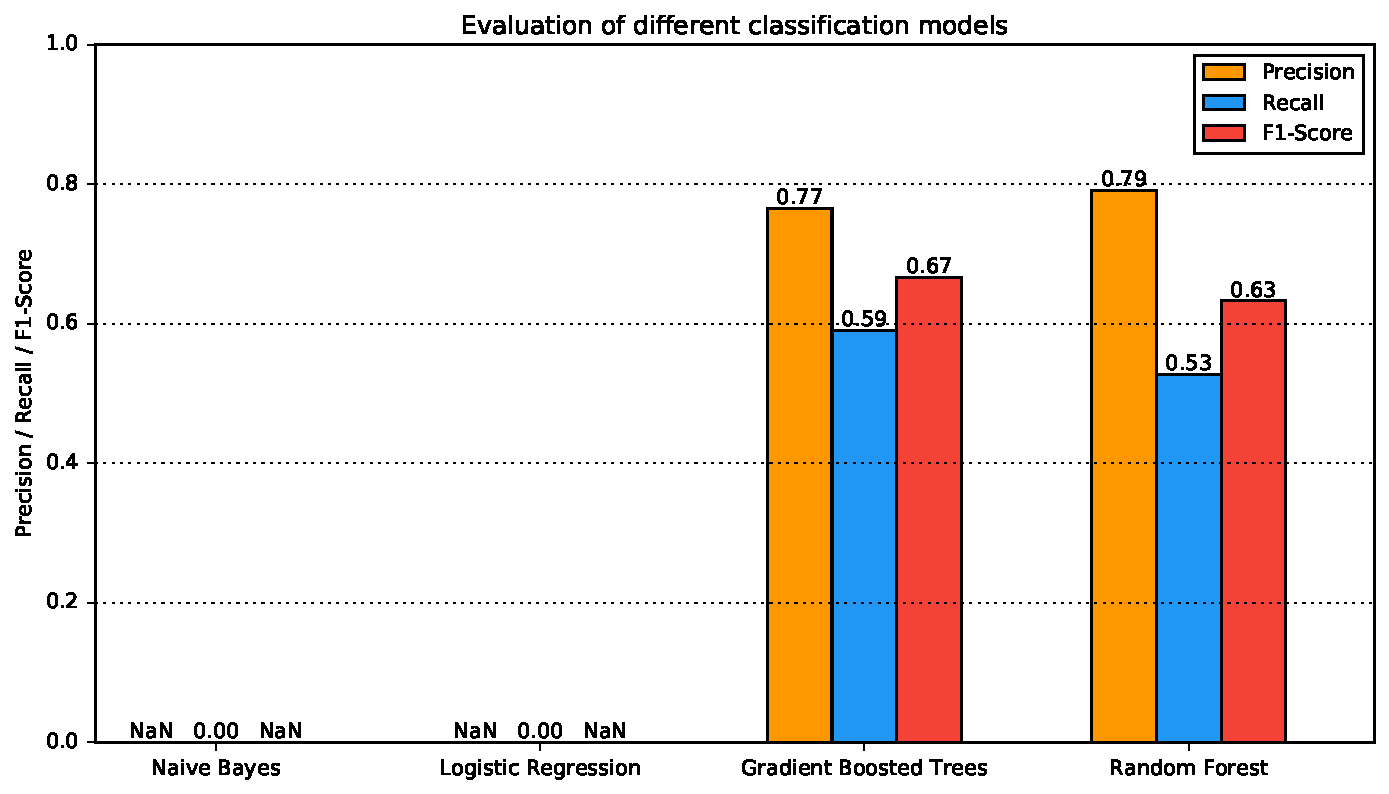
\includegraphics[width=0.9\textwidth]{img/classifier_eval}
	\caption{Evaluation of different classification models.}
	\label{classifier_eval}
\end{figure}
The Naive Bayes and Logistic Regression were both tested with different thresholds for the classes. They were especially tested with thresholds heavily favoring the positive class to see whether or not they would classify anything as positive. Unfortunately, this did not result in a different classification result.\par
The same parameters concerning the Decision Trees were used for the Gradient Boosted Trees and the Random Forest. These were 20 trees, a maximum depth of 6 and a maximum of 40 bins. The Gradient Boosted Trees were tested with a few different number of iterations. The values displayed in Figure \ref{classifier_eval} were the best for the tested number of iterations, which were 20. The other values resulted in a minimally worse Precision. The number of trees, the maximum depth and the maximum number of bins were tested using a Random Forest, but none of these parameters changed anything significantly.\par

\subsection{Class Threshold Evaluation}
The class thresholds can be, as previously described, used to favor one class over the other. Since the Spark MLlib does not provide a way to change the class thresholds or the loss function for Gradient Boosted Trees the evaluation of the class thresholds was done only with a Random Forest. Figure \ref{rf_thresh_large} shows the behavior of the quality measures with a different threshold. A threshold $> 1$ means that the class positive is favored and a threshold $< 1$ means that the class negative is favored. The relative distance signifies how strong a class is favored, i.e. a threshold of $0.5$ favors the class negative as much as a threshold of $2.0$ favors the class positive.\par
\begin{figure}[H]
	\centering
	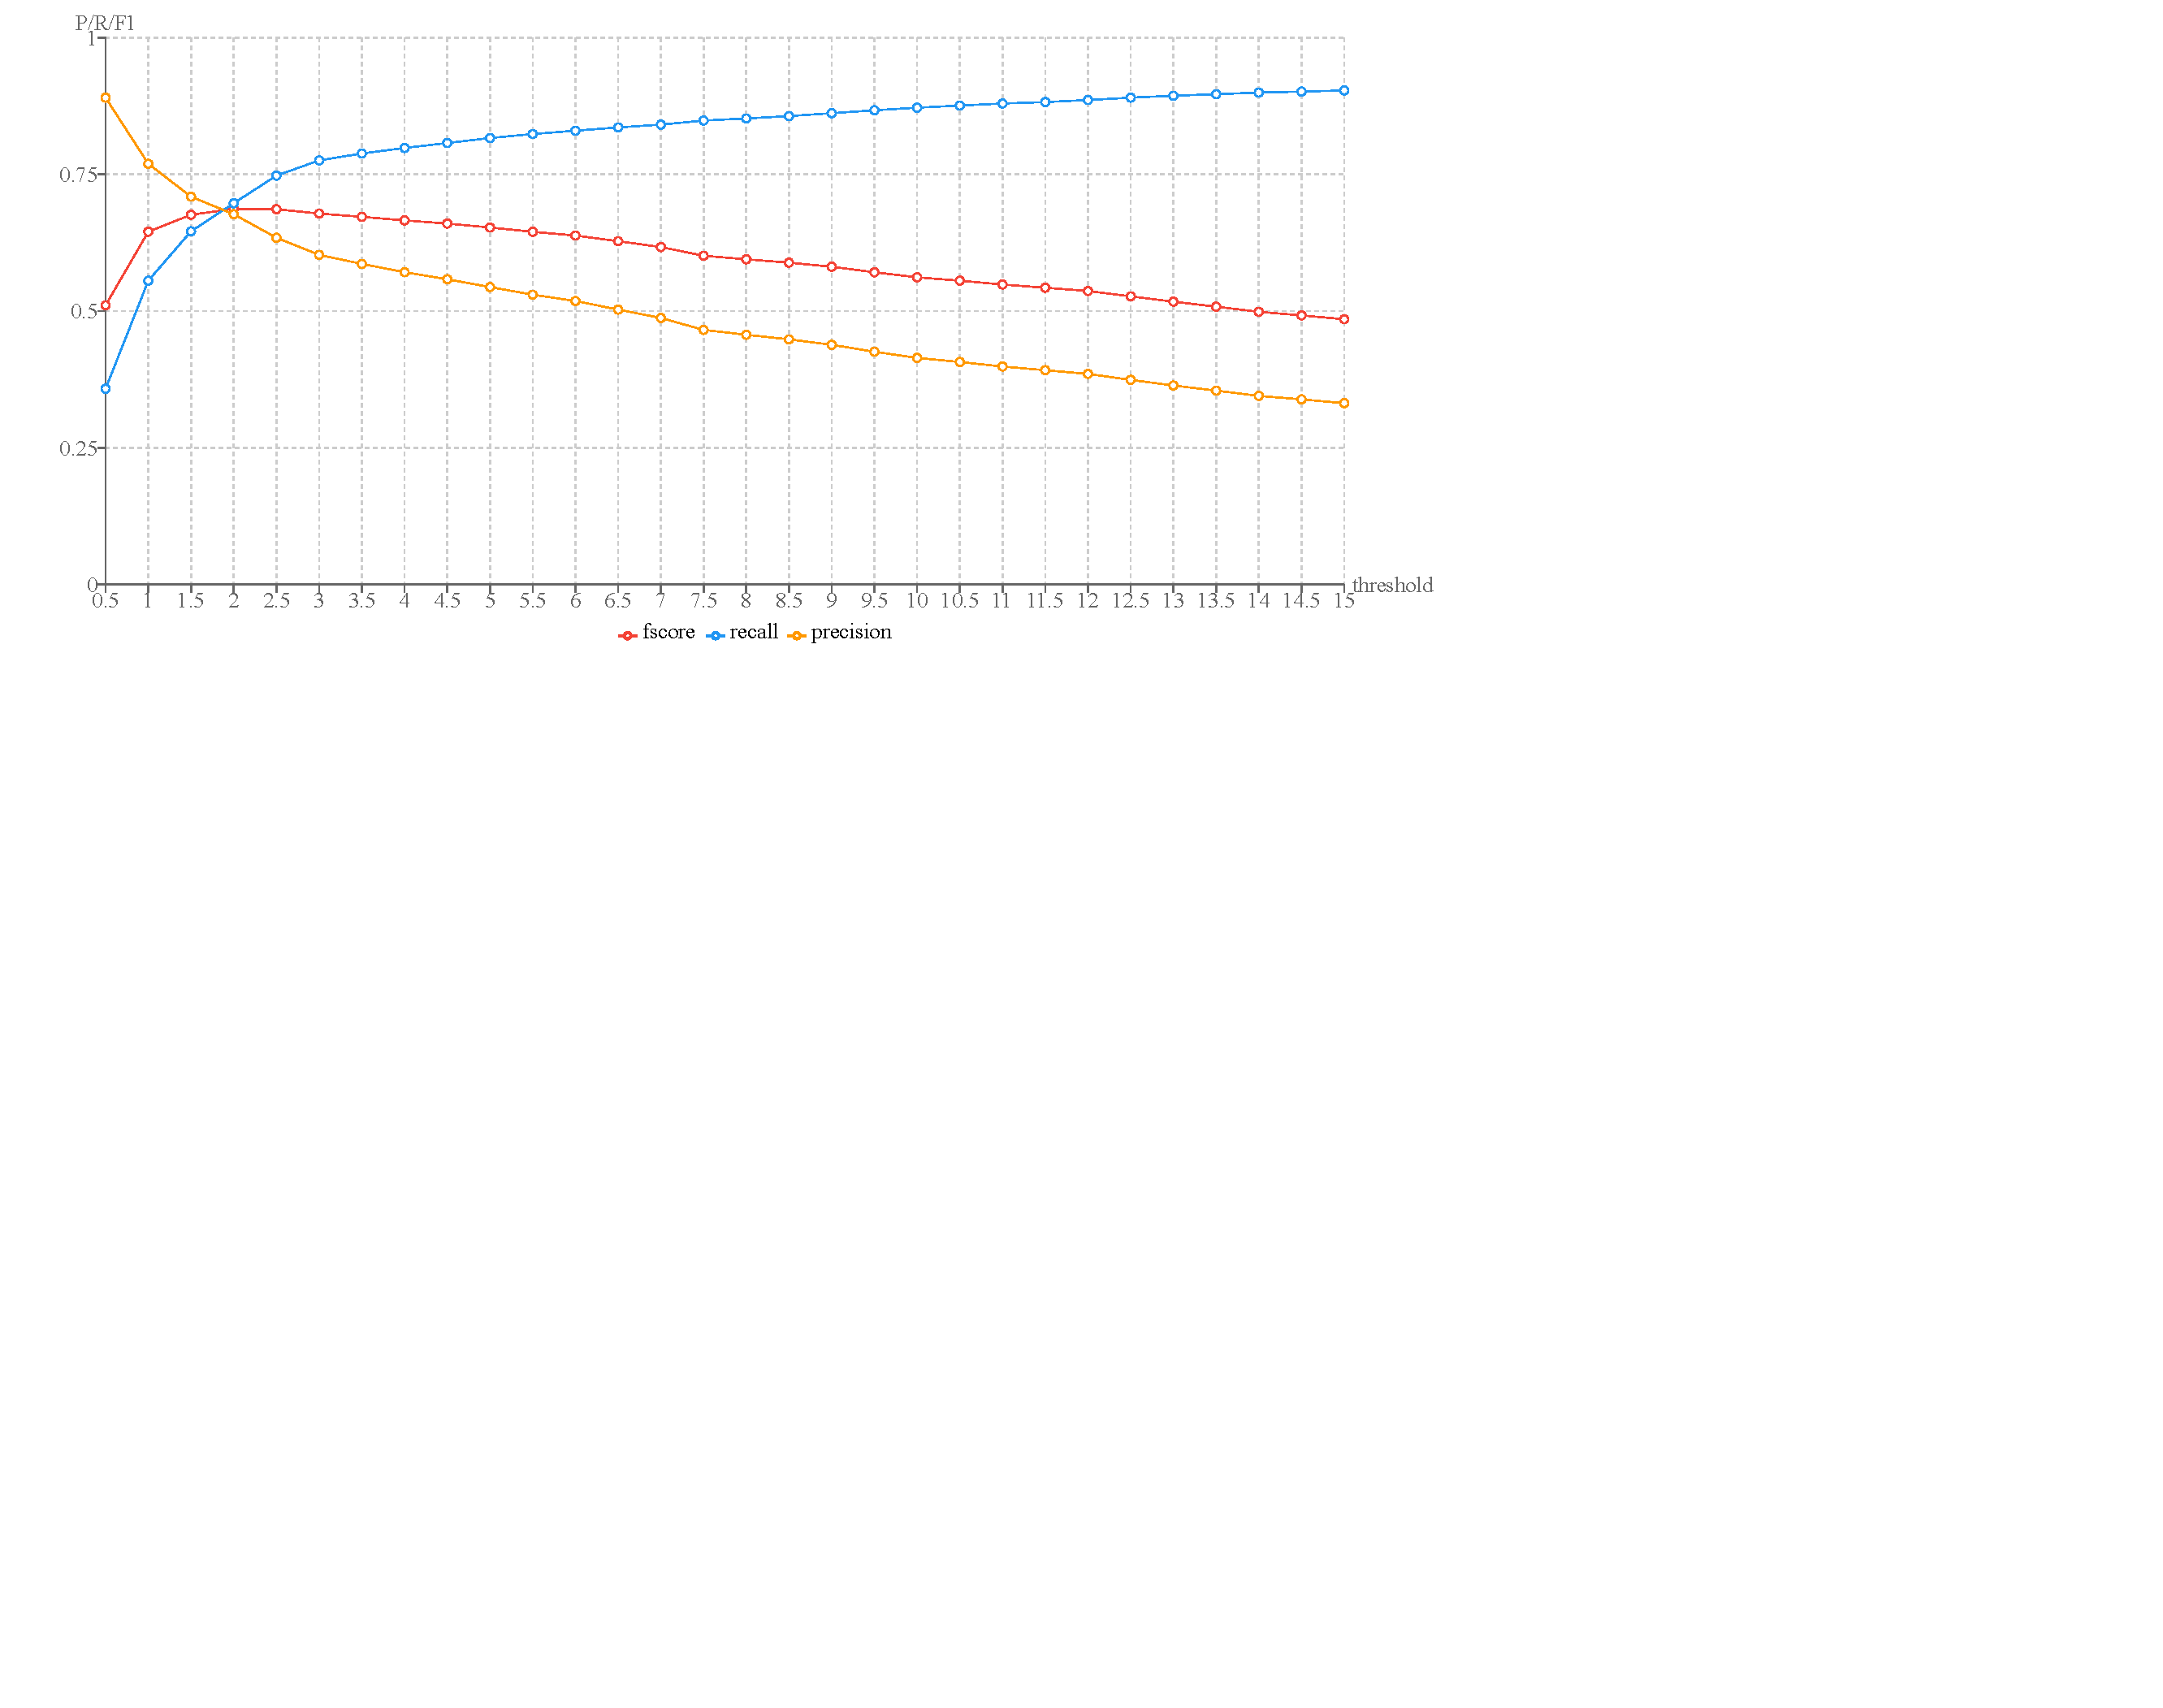
\includegraphics[width=0.9\textwidth]{img/rf_thresh_large}
	\caption{Evaluation of different class thresholds of a random forest model.}
	\label{rf_thresh_large}
\end{figure}
It is visible that a low threshold results in a very high precision with a relatively low recall. The threshold of $0.5$ results in a Precision of $89\%$ and a Recall of $36\%$. A very high threshold leads to a higher Recall with a worse Precision. An $80\%$ Recall is achieved with a threshold of $4$, which has a Precision of $57\%$. A $90\%$ Recall is achieved with a threshold of $14.5$, which has a Precision of $34\%$. This shows that increasing the threshold has diminishing returns for the Recall while the drop of the Precision is relatively uniform.\par
Adjusting the thresholds produces indeed a high Precision and a high Recall classifier, which in the future can be used to create the high-quality seed and high-coverage candidate alignments presented by Grütze et al. \cite{coheel}. The candidate alignments would be used to increase the Recall of the seed alignments, e.g. by using Random Walks.\par

\subsection{Comparison with realistic Quality Measure}
The adjusted quality measures take the collisions described in Section \ref{sec:NEL} into account. These are an adjusted Precision and an adjusted Recall. They are calculated the same way the normal Precision and Recall are calculated but use different sets for the calculation.\par
Let the set $U \subset T$ contain all feature entries, which were the only ones classified as positive for its alias, i.e. there is no collision. $U$ is then used to remove all feature entries with collisions. Let $T'_{TP} = T_{TP} \cap U$ and $T'_{FP} = T_{FP} \cap U$. The feature entries producing collisions are then added to $T_{FN}$: $T'_{FN} = T_{FN} \cup (T_{TP} - U) \cup (T_{FP} - U)$. The sets $T'_{TP}$, $T'_{FP}$ and $T'_{FN}$ are then used to calculate Precision, Recall and $F_1$-Score.\par
\begin{figure}[H]
	\centering
	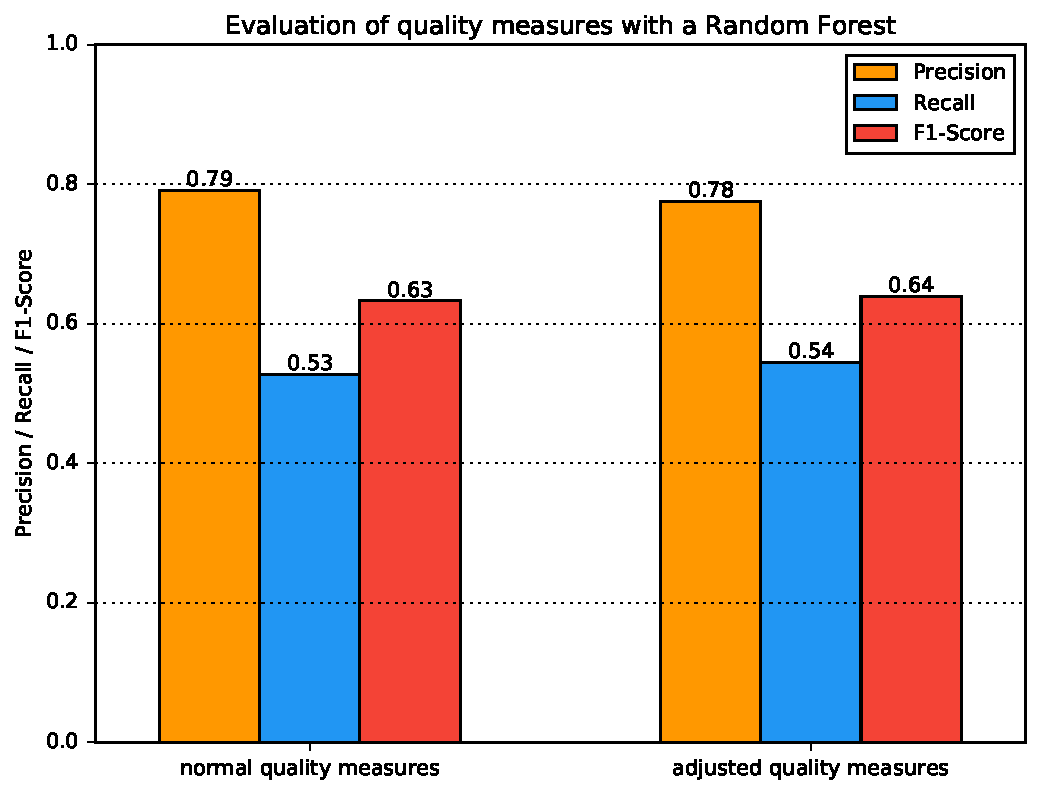
\includegraphics[width=0.7\textwidth]{img/qualitymeasure_eval}
	\caption{Evaluation of quality measures.}
	\label{qualitymeasure_eval}
\end{figure}
Figure \ref{qualitymeasure_eval} shows that while taking the collisions into account the Precision drops only by one per cent. This proves that the classifier does not produce a lot of collisions and, therefore, the original quality measures are accurate enough to properly evaluate the classification models in this section and the features in the next section.

% Kurz erklären was man im Bild sieht\par
% Naive Bayes
% \begin{itemize}
% 	\item nimmt an die features seien unabhängig, was sie nicht sind
% 	\item sagt immer nein, da zu viele negative feature entries
% 	\item verschiedene Kostenmodelle/Gewichte getestet
% \end{itemize}
% Logistic Regression
% \begin{itemize}
% 	\item sagt immmer nein, da zu viele negative feature entries
% 	\item verschiedene Kostenmodelle getestet
% 	\item Standard Paramter der Spark ML lib (und des Beispiels) benutzt
% \end{itemize}
% Gradient Boosted Trees
% \begin{itemize}
% 	\item benutzte parameter
% 	\item Bei Iteration Parameter den minimal besten Wert bei 20 Iterationen (ein paar verschiedene Iterationen getestet)
% \end{itemize}
% Random Forest
% \begin{itemize}
	% \item vergleich DF und RDD API
% 	\item parameter getuned, haben aber nicht wirklich was geändert
% 	\item Kostenmodell kurve zeigen (für Seed und Candidate Alignments)
% \end{itemize}


% \begin{figure}[H]
% 	\centering
% 	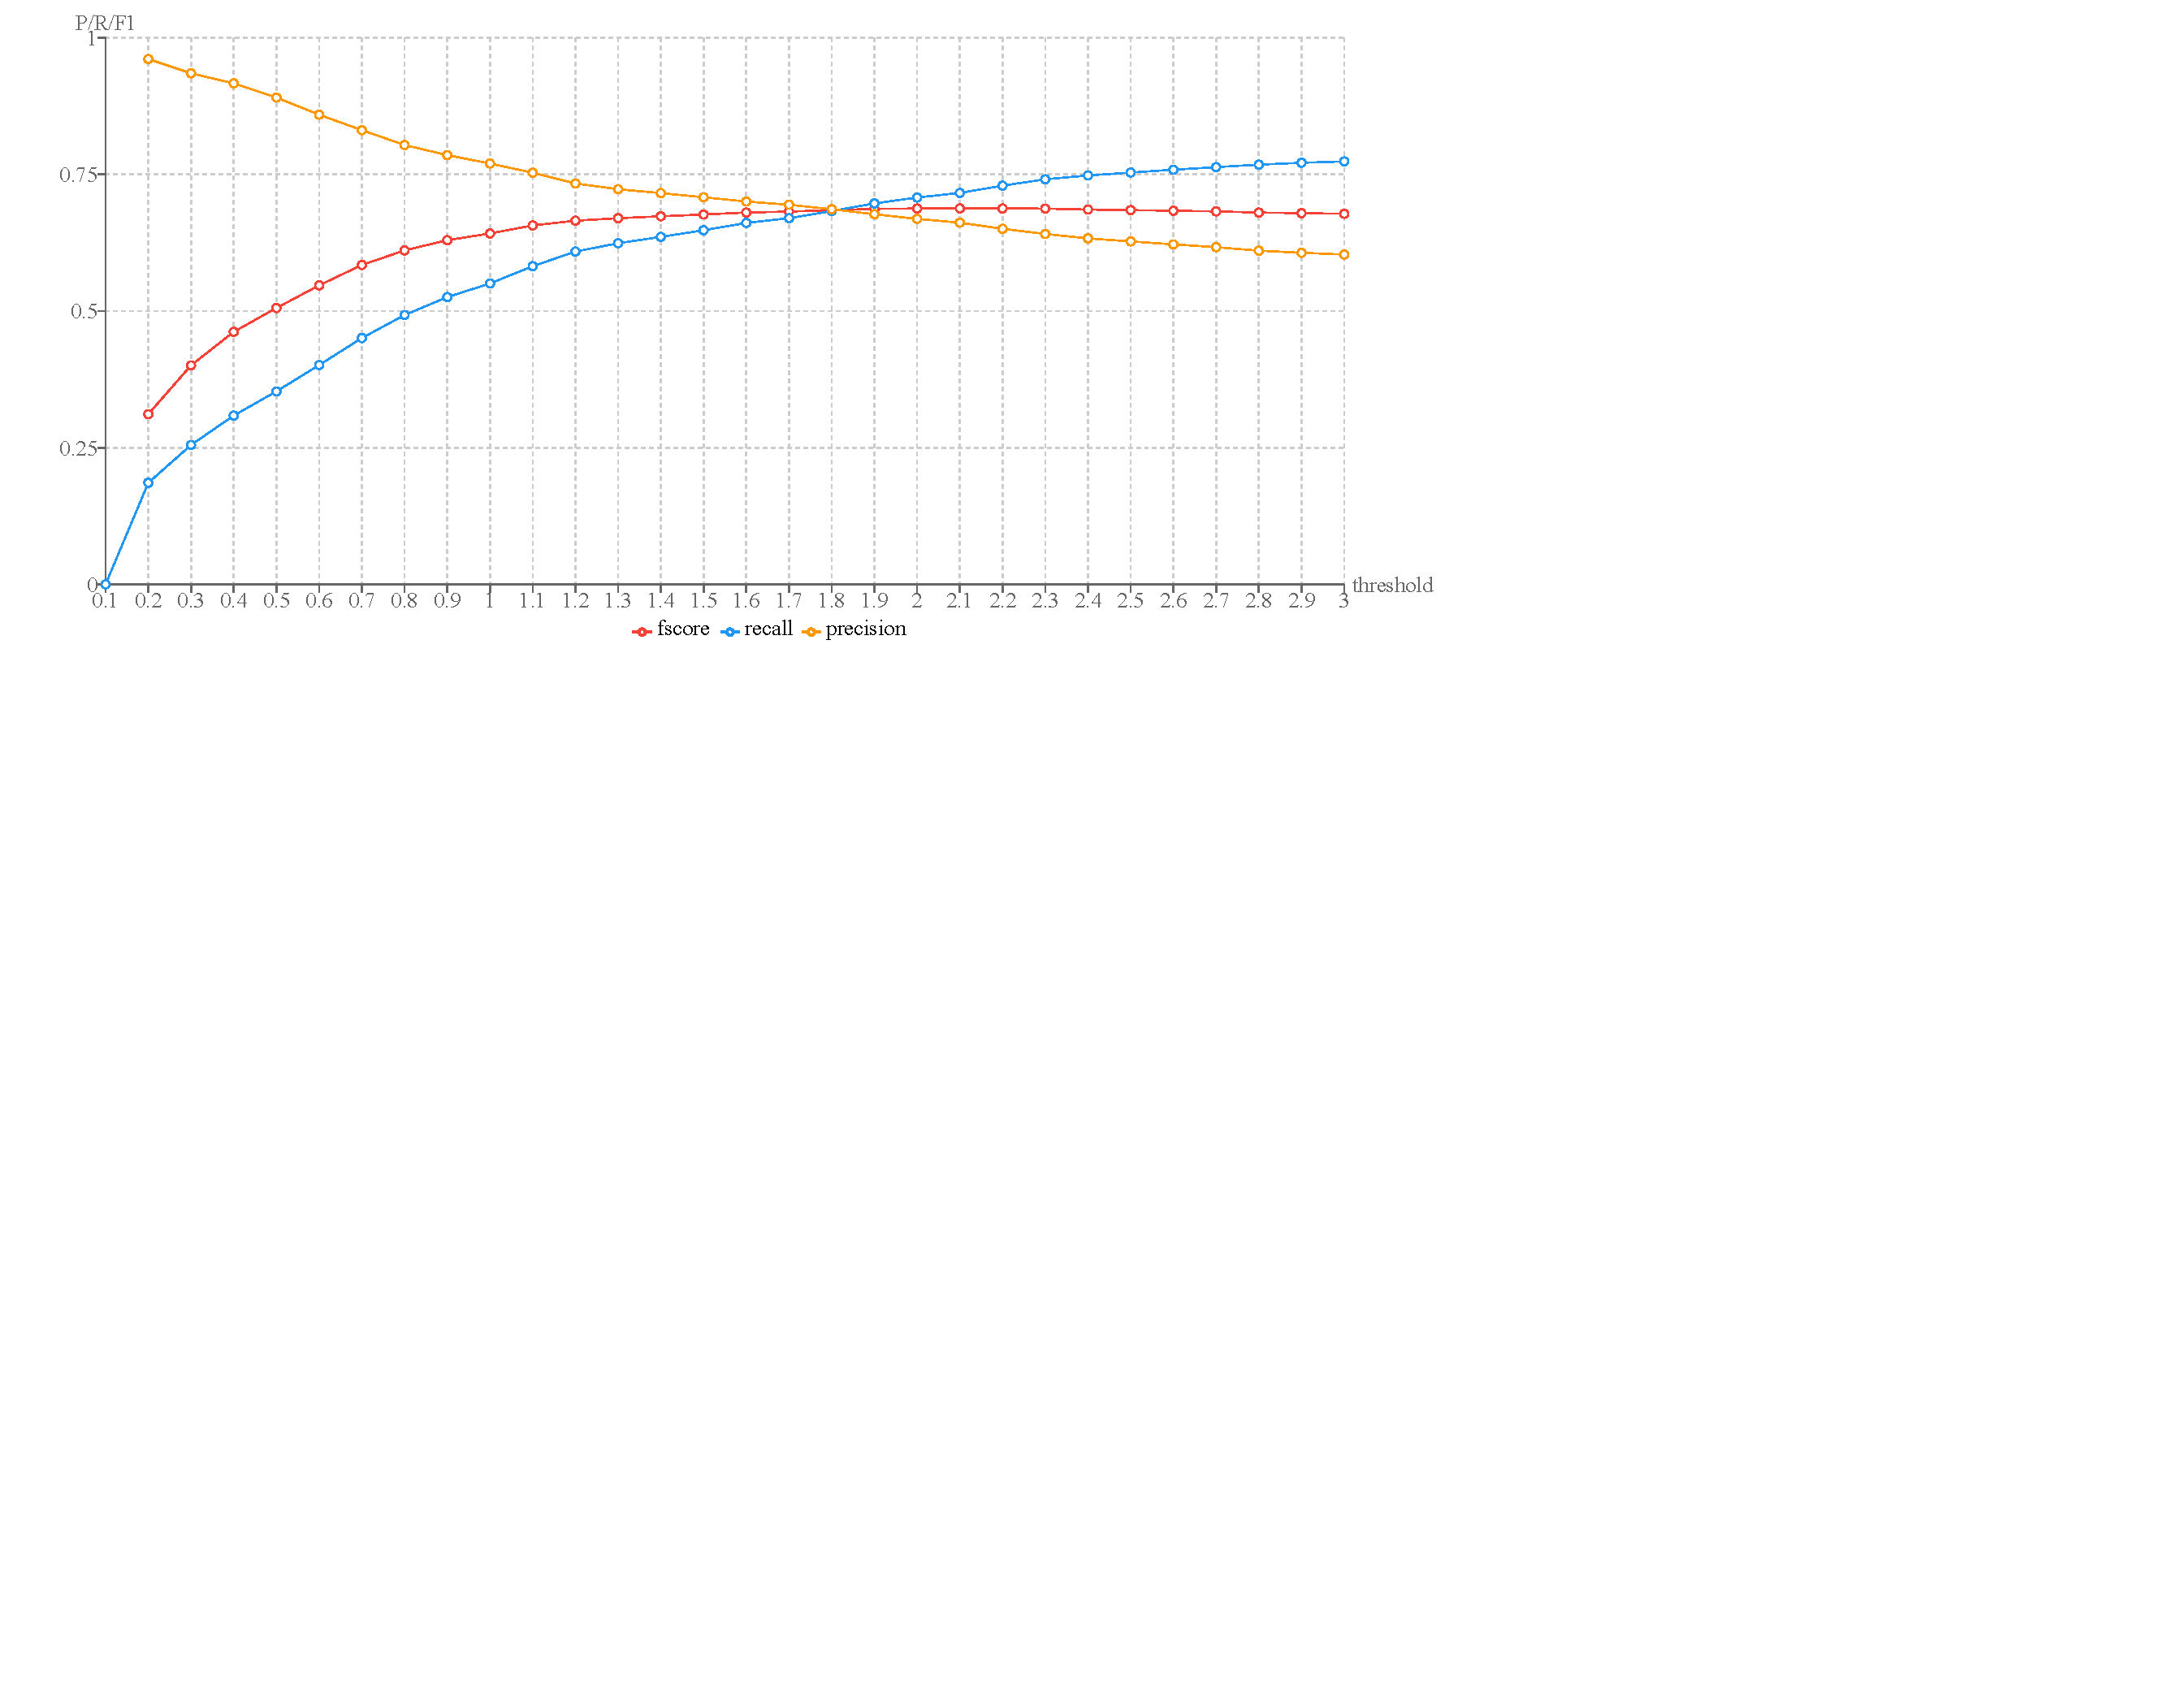
\includegraphics[width=\textwidth]{img/rf_thresh_small}
% 	\caption{Evaluation of different class weights of a random forest model.}
% 	\label{rf_thresh_small}
% \end{figure}
\newpage
\section{Evaluation of the first and higher order features (2-3 Seiten)}
\begin{itemize}
	\item mit welchem Classifier getestet
	\item Parameter des Classifiers auch erwähnen
	\item erklären, warum keine exhaustive grid search (dauert zu lange)
	\item Training- und Testvorgang beschreiben (ist wie in der section davor)
	\item benutzen auch die gleichen Evaluierungsmaße
	\item eine "Control-Group" haben (mit allen Features)
\end{itemize}

	\subsection{Link Score}
	\subsection{Page Score}
		\subsubsection{Rank}
		\subsubsection{Delta Top}
		\subsubsection{Delta Successor}
	\subsection{Context Score}
		\subsubsection{Rank}
		\subsubsection{Delta Top}
		\subsubsection{Delta Successor}

\newpage
% (1 Seite)
\section{NEL on Newspaper Articles}
\label{sec:NELEval}
This section discusses the impact of different training data on and the performance of the presented NER and EL approach when annotating German newspaper articles. The documents were annotated on an eight node cluster using Apache Spark. Each node has a 6-Core CPU with 2.4 GHz and 64GB of RAM.\par

\subsection*{Impact of different Training Sets}
When the classifier is trained using only feature entries generated by links the resulting annotations contain a lot of false annotations. The inclusion of the trie aliases makes the classifier a lot more cautious by providing many occasions, where the alias is not linked at all. But this also adds many more feature entries and thereby increases the duration needed to train the model. It also adds so many negative entries that even Decision Tree models classify every feature entry as negative. The training set used in Section \ref{sec:ModelEval} and \ref{sec:FeatureEval} contains a total of 1.8 million positive feature entries and 545.9 million negative feature entries. When removing all feature entries with a rank $\geq 10$ the around 548 million feature entries are reduced to only 25.3 million. To preserve realistic Precision and Recall only the training data is filtered. Mainly negative feature entries are removed this way, which, therefore, fixes the problem of only negative predictions.\par
The selection of the Wikipedia pages used to generate the training data also influences the quality of the classifier. The Precision and Recall are not affected that strongly but the annotation results vary greatly. Using all Wikipedia pages of businesses, which are around $1.5\%$ of all pages, results in better annotation results than using a random $1\%$ sample of pages. This is caused by the pages of businesses having, on average, more links than a random page and generally linking more to other businesses.\par

\subsection*{Performance}
The annotation of newspaper articles contains two steps. The first step is the generation of feature entries and the second the classification of those. The generation of the feature entries costs most of the time while the classification performs extremely well. The annotation of 3.6 million Wikipedia pages took 27 hours. As a comparison, the classification of 126 million feature entries, generated from $1\%$ of Wikipedia pages, took only 2 minutes. The performance of the feature generation could be improved in the future by storing the documents in a more storage efficient way. An example would be using a global word dictionary for all words and storing the indices for each word in a document. The current performance of the document annotation is still good and it is possible, as shown, to annotate millions of documents in an acceptable amount of time. One big advantage of this performance is the possibility to e.g. annotate newly published newspaper articles daily. This would regularly enrich the knowledge base of businesses with new relations and thus keep it up to date.\par

% % Discussion
% 	\subsection{Inclusion of Trie Aliases}
% 	\begin{itemize}
% 		\item warum überhaupt benutzt: Negatives in den Trainingsdaten (also gefundenes Mention ohne Alignment)
% 		\item entfernen der Füllwörter
% 		\item vergleichen mit einfachem Stopword und Symbol filtern
% 		\item Rechenkosten (wieviele Positives und Negatives es gibt)
% 	\end{itemize}
% 	\subsection{Impact of different Training Sets}
% 	\begin{itemize}
% 		\item Unterschied verschiedener Artikel als Trainingsdaten
% 		\item was wurde bei welchen Trainingsdaten verlinkt
% 	\end{itemize}
% 	\subsection{Andere Quality Measures}
% 	\begin{itemize}
% 		\item Anderere precision recall fscore vergleichen
% 	\end{itemize}
% 	\subsection{Performance}
% 	\begin{itemize}
% 		\item mit welcher Hardware haben wir gearbeitet
% 		\item Dauer des Trainings mit wievielen Dateneinträgen
% 		\item Dauer des NEL auf Wikipedia und Spiegel Online
% 	\end{itemize}
% 	\subsection{Results on Spiegel Online}
% 	\begin{itemize}
% 		\item sind die Links benutzbar
% 		\item einen Auszug zeigen
% 		\item aggregieren auf welche Entitäten wie oft verlinkt wurde
% 	\end{itemize}
\newpage
% (1 Seite)
\section{Conclusion}
\label{sec:Conclusion}
We presented an approach that combines both NER and EL and performs both in an efficient way. It is a practical solution as it is possible to annotate millions of documents in an acceptable amount of time. It annotated 3.6 million German Wikipedia articles in only 27 hours. With such a performance it is possible to annotate newly published newspaper articles in real-time. That way it is possible to extract relations from these annotated documents in real time and keep the knowledge base up to date.\par
We used Apache Spark on an eight node cluster, as described in Section \ref{sec:NELEval}, to annotate the documents on a distributed system. Apache Spark scales horizontally, which means that to increase the performance only new nodes need to be added to the cluster. This is a very cost efficient way to scale since the nodes don't need top of the line hardware.\par
The combined NER and EL achieves a high Precision of $90\%$. The Recall can be increased to $80\%$ if required at the cost of some Precision. This is achieved by adjusting the class thresholds of the classification model as described in Section \ref{sec:ModelEval}. These Precision and Recall values contain both NER and EL, which are both not easily solved. Additionally, the presented approach annotates unstructured German texts, which are harder to annotate due to the German language being more complex than English.\par
There are a few ways to improve the performance and the quality of the presented approach. One way to increase the performance would be to decrease the memory footprint of the documents by using more memory efficient ways to encode them. This would increase the scalability of the feature generation, which takes up most of the time. The quality of the classification could be increased by combining a high Precision and a high Recall model as proposed by Grütze et al. \cite{coheel}. The current approach can be used to create both a high Precision and high Recall classifier by adjusting the class thresholds. These could then be combined by using e.g. Random Walks to increase the Recall of the high Precision classifier without hurting the Recall.

	% \subsection*{Achievements}
	% \begin{itemize}
	% 	\item sind die neuen Links benutzbar
	% 	\item eine Statisik der verlinkten Artikel vielleicht
	% 	\item können aus den getaggten Artikel Relationen extrahiert werden
	% 	\item können Millionen von Artikeln in Stunden verlinken (auch in CohEEL erwähnt)
	% \end{itemize}

	% \subsection*{Possible Improvements}
	% \begin{itemize}
	% 	\item verbessern der Links durch die in CohEEL benutzen Random Walks mit den Candidate Alignments
	% 	\item Blacklist Trie um schlechte/falsche Mentions zu verhindern
	% \end{itemize}


\newpage
\addcontentsline{toc}{section}{References}
% BibTeX Styles nach Norm DIN 1505
\bibliographystyle{plaindin}
\bibliography{bibfile}
\newpage
\addcontentsline{toc}{section}{Glossary}
\section*{Glossary}
NEL - Named entity linking
\newpage
\section*{Statutory Declaration}
I declare that I have written this thesis independently, that I have not used any other than the declared resources, and that I have explicitly marked all material which has been quoted either literally or by content from the used sources.

Potsdam, \today
~\\
~\\
~\\
\sign{Jan Ehmüller}


\end{document}
